\section{ListGraphVisitor Class Reference}
\label{classListGraphVisitor}\index{ListGraphVisitor@{ListGraphVisitor}}
{\tt \#include $<$ListGraphVisitor.h$>$}



\subsection{Detailed Description}
This class list the node in the order they would be encountered depth first and builds a formatted string using newline and tab characters to show the structure of the graph it follows a variant of the visitor desing pattern. 

Definition at line 23 of file ListGraphVisitor.h.\subsection*{Public Member Functions}
\begin{CompactItemize}
\item 
{\bf ListGraphVisitor} (boost::shared\_\-ptr$<$ {\bf SceneGraph} $>$ graph)
\begin{CompactList}\small\item\em constructor \item\end{CompactList}\item 
{\bf $\sim$ListGraphVisitor} (void)
\begin{CompactList}\small\item\em destructor \item\end{CompactList}\item 
void {\bf discover\_\-vertex} ({\bf vertex\_\-descriptor} v, const {\bf graph\_\-type} \&g)
\begin{CompactList}\small\item\em \begin{Desc}
\item[Parameters:]
\begin{description}
\item[{\em v}]a vertex index which points to which vertex/node is discovered \end{description}
\end{Desc}
\item\end{CompactList}\item 
void {\bf finish\_\-vertex} ({\bf vertex\_\-descriptor} v, const {\bf graph\_\-type} \&g)
\begin{CompactList}\small\item\em \begin{Desc}
\item[Parameters:]
\begin{description}
\item[{\em v}]a vertex index which points to which vertex/node is discovered \end{description}
\end{Desc}
\item\end{CompactList}\item 
std::string {\bf getGraphList} (void)
\begin{CompactList}\small\item\em \begin{Desc}
\item[Returns:]the formatted string of the graph \end{Desc}
\item\end{CompactList}\end{CompactItemize}
\subsection*{Data Fields}
\begin{CompactItemize}
\item 
std::vector$<$ boost::default\_\-color\_\-type $>$ {\bf T}
\begin{CompactList}\small\item\em a color map required by the depth first traversal algorithm \item\end{CompactList}\end{CompactItemize}


\subsection{Constructor \& Destructor Documentation}
\index{ListGraphVisitor@{ListGraphVisitor}!ListGraphVisitor@{ListGraphVisitor}}
\index{ListGraphVisitor@{ListGraphVisitor}!ListGraphVisitor@{ListGraphVisitor}}
\subsubsection{\setlength{\rightskip}{0pt plus 5cm}ListGraphVisitor::ListGraphVisitor (boost::shared\_\-ptr$<$ {\bf SceneGraph} $>$ {\em graph})\hspace{0.3cm}{\tt  [inline]}}\label{classListGraphVisitor_979dcaa51c8861959024ded62b97937d}


constructor 



Definition at line 41 of file ListGraphVisitor.h.\index{ListGraphVisitor@{ListGraphVisitor}!$\sim$ListGraphVisitor@{$\sim$ListGraphVisitor}}
\index{$\sim$ListGraphVisitor@{$\sim$ListGraphVisitor}!ListGraphVisitor@{ListGraphVisitor}}
\subsubsection{\setlength{\rightskip}{0pt plus 5cm}ListGraphVisitor::$\sim$ListGraphVisitor (void)\hspace{0.3cm}{\tt  [inline]}}\label{classListGraphVisitor_ce76d0b68b0ea97e3792400872347877}


destructor 



Definition at line 55 of file ListGraphVisitor.h.

\subsection{Member Function Documentation}
\index{ListGraphVisitor@{ListGraphVisitor}!discover\_\-vertex@{discover\_\-vertex}}
\index{discover\_\-vertex@{discover\_\-vertex}!ListGraphVisitor@{ListGraphVisitor}}
\subsubsection{\setlength{\rightskip}{0pt plus 5cm}void ListGraphVisitor::discover\_\-vertex ({\bf vertex\_\-descriptor} {\em v}, const {\bf graph\_\-type} \& {\em g})\hspace{0.3cm}{\tt  [inline]}}\label{classListGraphVisitor_435686d2ecb09466647032db850584c3}


\begin{Desc}
\item[Parameters:]
\begin{description}
\item[{\em v}]a vertex index which points to which vertex/node is discovered \end{description}
\end{Desc}


\begin{Desc}
\item[Parameters:]
\begin{description}
\item[{\em g}]a reference to the graph being traversed this method is called by the depth first traversal algorithm every time a node is discovered it builds the graph string as a stream \end{description}
\end{Desc}


Definition at line 66 of file ListGraphVisitor.h.\index{ListGraphVisitor@{ListGraphVisitor}!finish\_\-vertex@{finish\_\-vertex}}
\index{finish\_\-vertex@{finish\_\-vertex}!ListGraphVisitor@{ListGraphVisitor}}
\subsubsection{\setlength{\rightskip}{0pt plus 5cm}void ListGraphVisitor::finish\_\-vertex ({\bf vertex\_\-descriptor} {\em v}, const {\bf graph\_\-type} \& {\em g})\hspace{0.3cm}{\tt  [inline]}}\label{classListGraphVisitor_9d47bb532f76a2082b8343273cefd63d}


\begin{Desc}
\item[Parameters:]
\begin{description}
\item[{\em v}]a vertex index which points to which vertex/node is discovered \end{description}
\end{Desc}


\begin{Desc}
\item[Parameters:]
\begin{description}
\item[{\em g}]a reference to the graph being traversed this method is called by the traversal algorithm whenever a vertex/node descandants have all been discovered it indicates that the traversal is backtracking \end{description}
\end{Desc}


Definition at line 84 of file ListGraphVisitor.h.\index{ListGraphVisitor@{ListGraphVisitor}!getGraphList@{getGraphList}}
\index{getGraphList@{getGraphList}!ListGraphVisitor@{ListGraphVisitor}}
\subsubsection{\setlength{\rightskip}{0pt plus 5cm}std::string ListGraphVisitor::getGraphList (void)\hspace{0.3cm}{\tt  [inline]}}\label{classListGraphVisitor_46a6ec7ac2284375c4ec816b5855c871}


\begin{Desc}
\item[Returns:]the formatted string of the graph \end{Desc}




Definition at line 93 of file ListGraphVisitor.h.

Referenced by BOOST\_\-AUTO\_\-TEST\_\-CASE().

Here is the caller graph for this function:\nopagebreak
\begin{figure}[H]
\begin{center}
\leavevmode
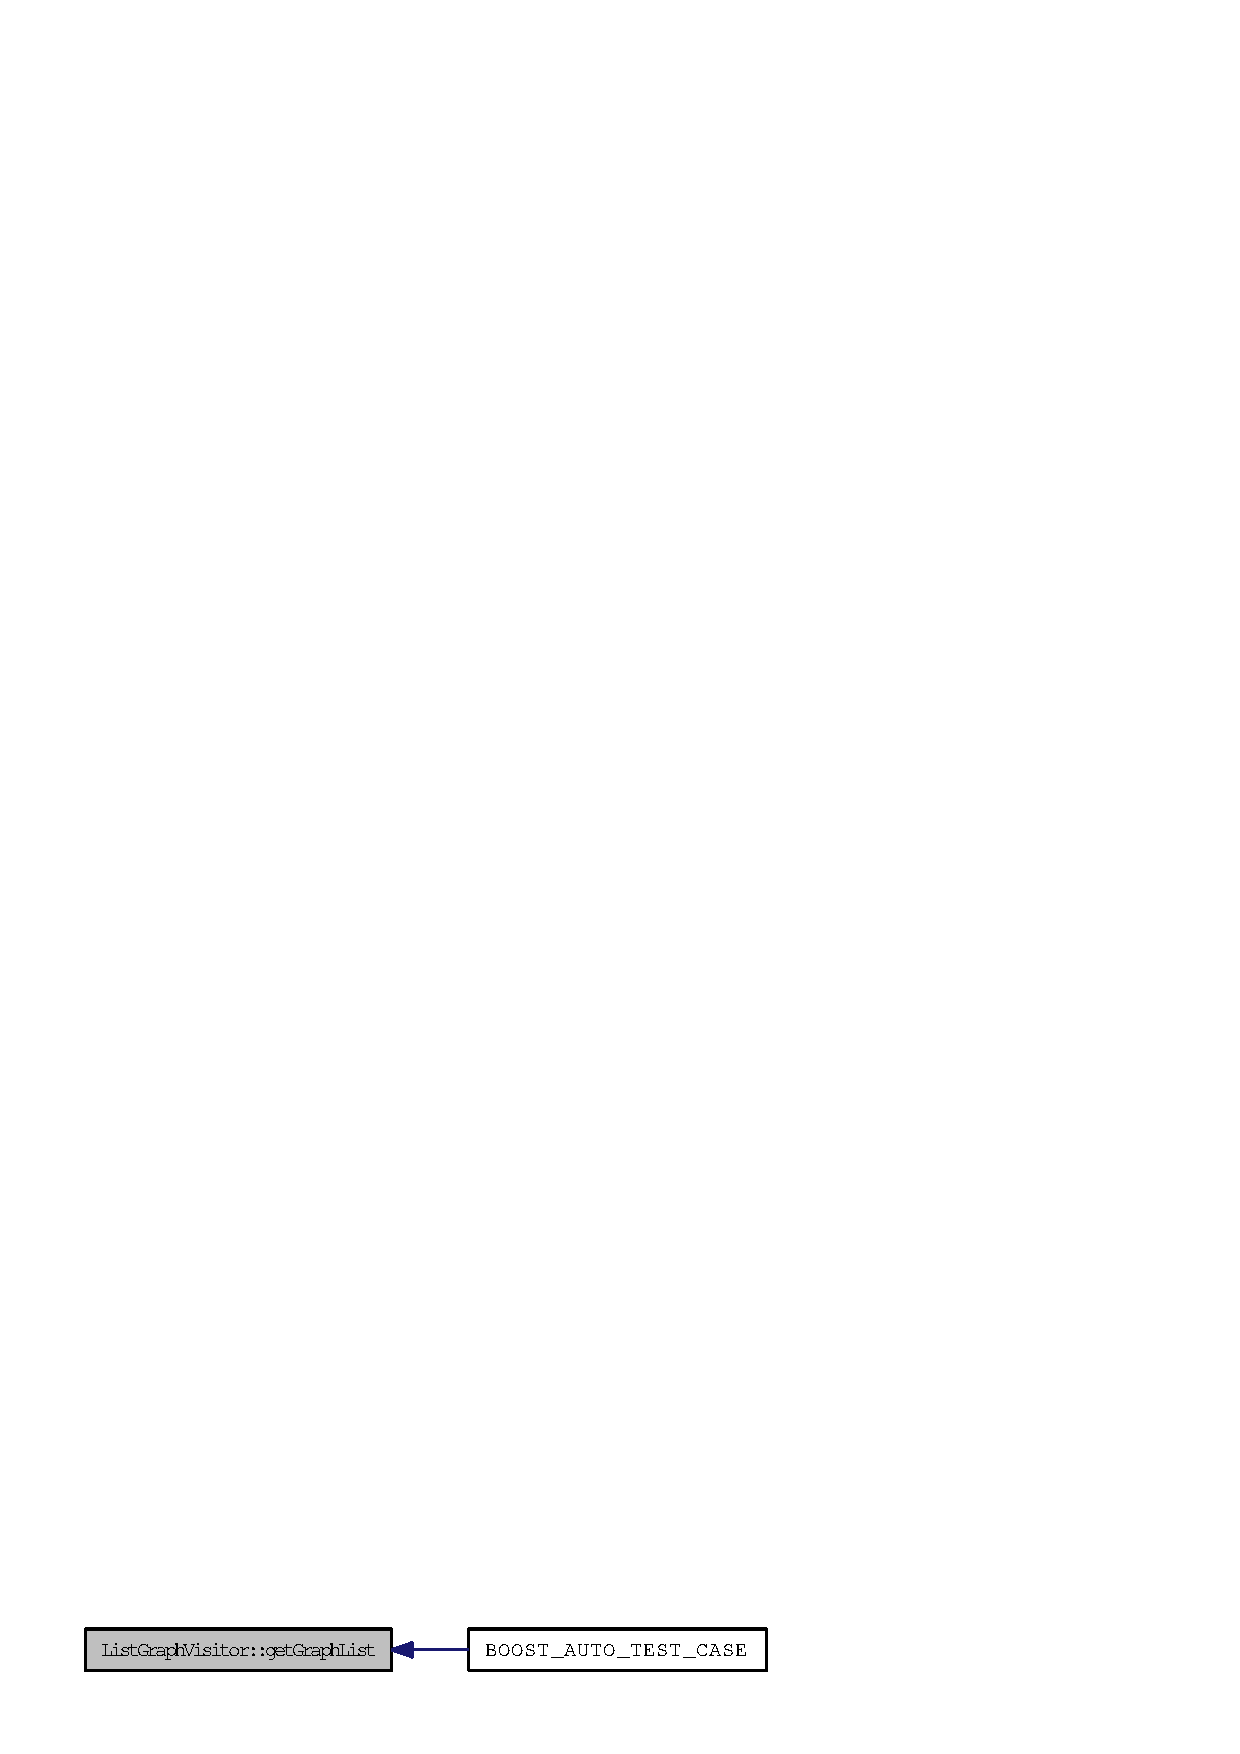
\includegraphics[width=186pt]{classListGraphVisitor_46a6ec7ac2284375c4ec816b5855c871_icgraph}
\end{center}
\end{figure}


\subsection{Field Documentation}
\index{ListGraphVisitor@{ListGraphVisitor}!T@{T}}
\index{T@{T}!ListGraphVisitor@{ListGraphVisitor}}
\subsubsection{\setlength{\rightskip}{0pt plus 5cm}std::vector$<$boost::default\_\-color\_\-type$>$ {\bf ListGraphVisitor::T}}\label{classListGraphVisitor_f0dbe8c9976400feef04e5cac95d0df1}


a color map required by the depth first traversal algorithm 



Definition at line 36 of file ListGraphVisitor.h.

The documentation for this class was generated from the following file:\begin{CompactItemize}
\item 
{\bf ListGraphVisitor.h}\end{CompactItemize}
